\section{Runtime View}
\subsection{Runtime Overview}
Dieser Abschnitt beschreibt die Laufzeitumgebung der Anwendung, einschließlich der genutzten Cloud-Ressourcen, Microservices und Datenbanken sowie deren Interaktionen.
Die Microservices werden in anwendungsweite Microservices, die von allen Tenants gemeinsam genutzt werden, und tenant-typ-spezifische Microservices unterteilt, die von allen Tenants eines bestimmten Tenant-Typs verwendet werden.
Ebenso erfolgt eine Unterteilung der Datenbanken in anwendungsweite und tenant-typ-spezifische Datenspeicher.

\begin{figure}[H]
	\centering
	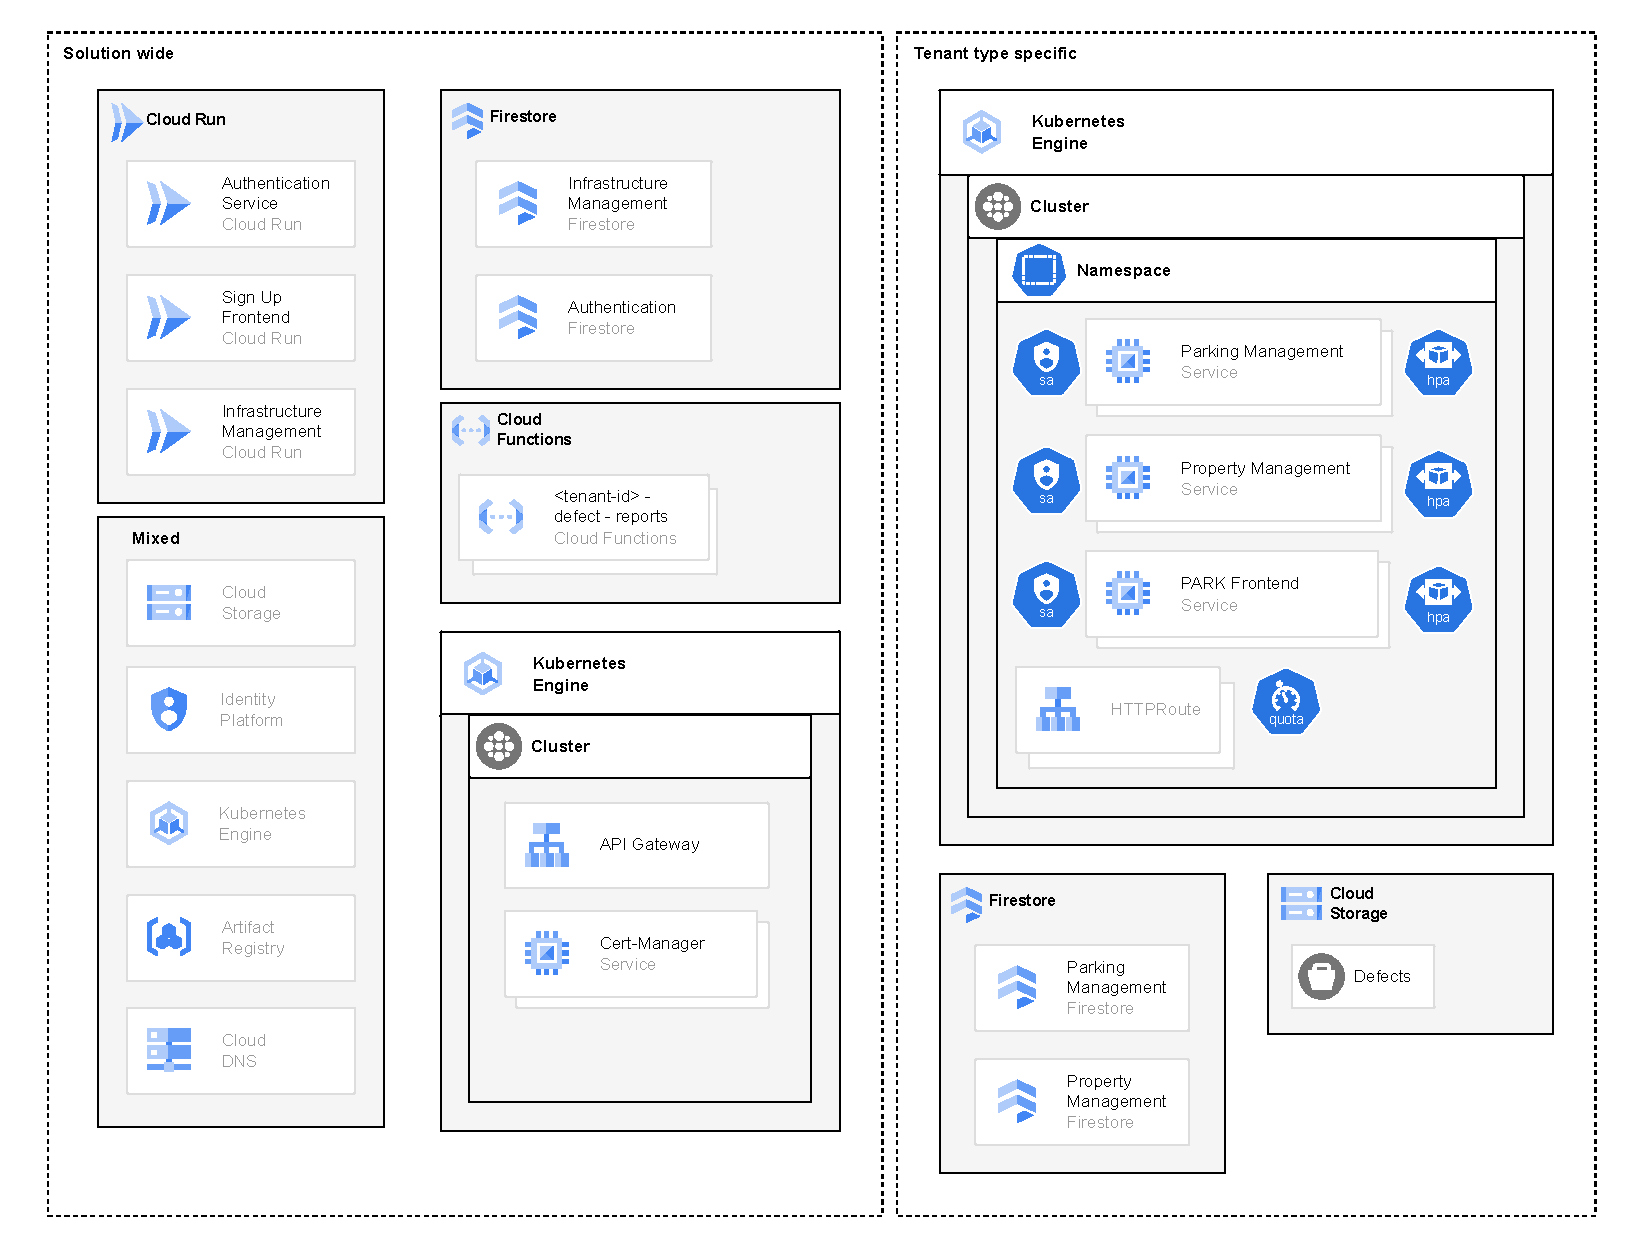
\includegraphics[width=\textwidth]{resources/03-runtime-view/pdf/cloud-ressources.pdf}
	\caption{Übersicht über die genutzten Cloud-Ressourcen}
	\label{fig:cloud-ressources}
\end{figure}

\begin{figure}[H]
	\centering
	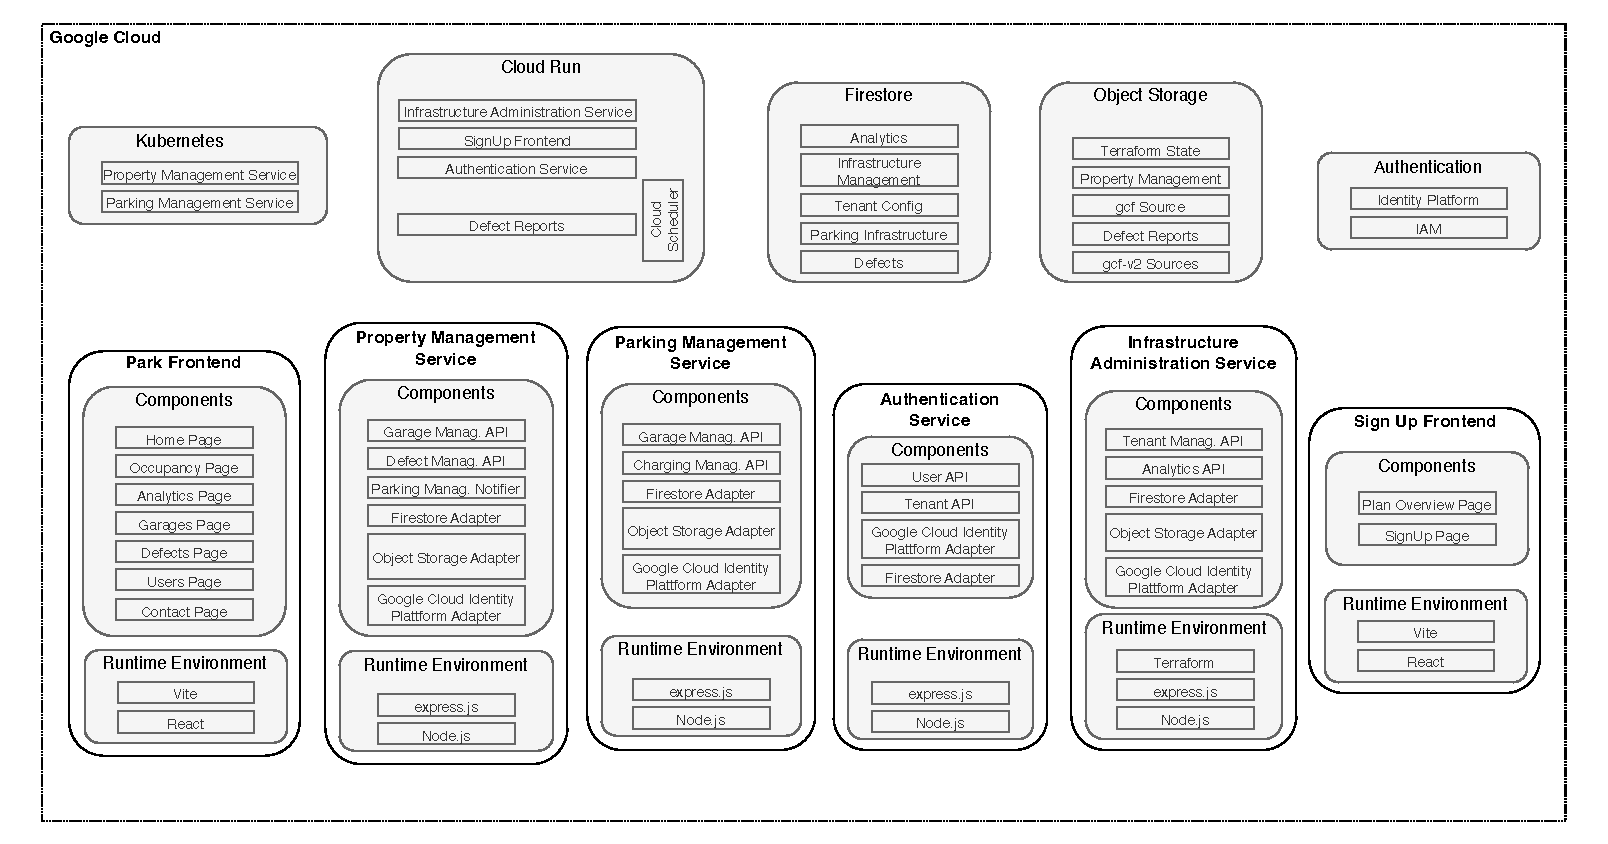
\includegraphics[width=\textwidth]{resources/03-runtime-view/pdf/architecture.pdf}
	\caption{Architekturübersicht der Microservices und deren zugehörige Cloud-Ressourcen}
	\label{fig:system-architecture}
\end{figure}

In Abbildung~\ref{fig:cloud-ressources} sind alle verwendeten Cloud-Ressourcen in zwei Kategorien unterteilt:
\paragraph{Globale Ressourcen}
Diese Ressourcen werden von allen Tenants gemeinsam genutzt und untergliedern sich in folgende Kategorien:
\begin{itemize}
	\item \textbf{Cloud Run} – Enthält alle Microservices, die in Cloud Run betrieben werden (Authentication Service, Infrastructure Management Service und Sign-Up Frontend).
	\item \textbf{Firestore} – Die Firestore-Datenbanken, die für die Cloud-Run-Services erforderlich sind.
	\item \textbf{Cloud Functions} – Jede Tenant-Instanz besitzt eine eigene Defect-Report Cloud Function.
	\item \textbf{Weitere Cloud-Ressourcen} – Sonstige Infrastrukturkomponenten wie Cloud Storage, Identity Platform, Kubernetes Engine, Artifact Registry sowie Ingress/DNS.
\end{itemize}

\paragraph{Tenant-Typ-spezifische Ressourcen}
Diese Ressourcen werden von allen Tenants desselben Tenant-Typs gemeinsam genutzt. Jeder Enterprise-Tenant wird als eigenständiger Typ betrachtet, um die verwendeten Ressourcen übersichtlich darzustellen. Die Ressourcen lassen sich in folgende Kategorien einteilen:
\begin{itemize}
	\item \textbf{Kubernetes} – Innerhalb der Kubernetes Engine existiert ein Cluster, in dem für jeden Tenant-Typ ein eigener Namespace angelegt wird. Innerhalb dieses Namespaces laufen die gemeinsam genutzten Services (Property Management Service, Parking Management Service).
	\item \textbf{Firestore} – Firestore-Datenbanken für die tenant-typ-spezifischen Services (Property Management Service, Parking Management Service).
	\item \textbf{Cloud Storage} – Eigene Buckets für den Property Management Service zur Speicherung von Defect-Bildern.
\end{itemize}

Zur Veranschaulichung der Interaktionen zwischen den Komponenten sowie den anwendungsweiten und tenant-typ-spezifischen Ressourcen zeigt Abbildung~\ref{fig:system-architecture} die vollständige Systemarchitektur. Hier ist zu erkennen, dass sich alle Komponenten eine Instanz des Authentication Service und des Infrastructure Management Service teilen.

\begin{figure}[H]
	\centering
	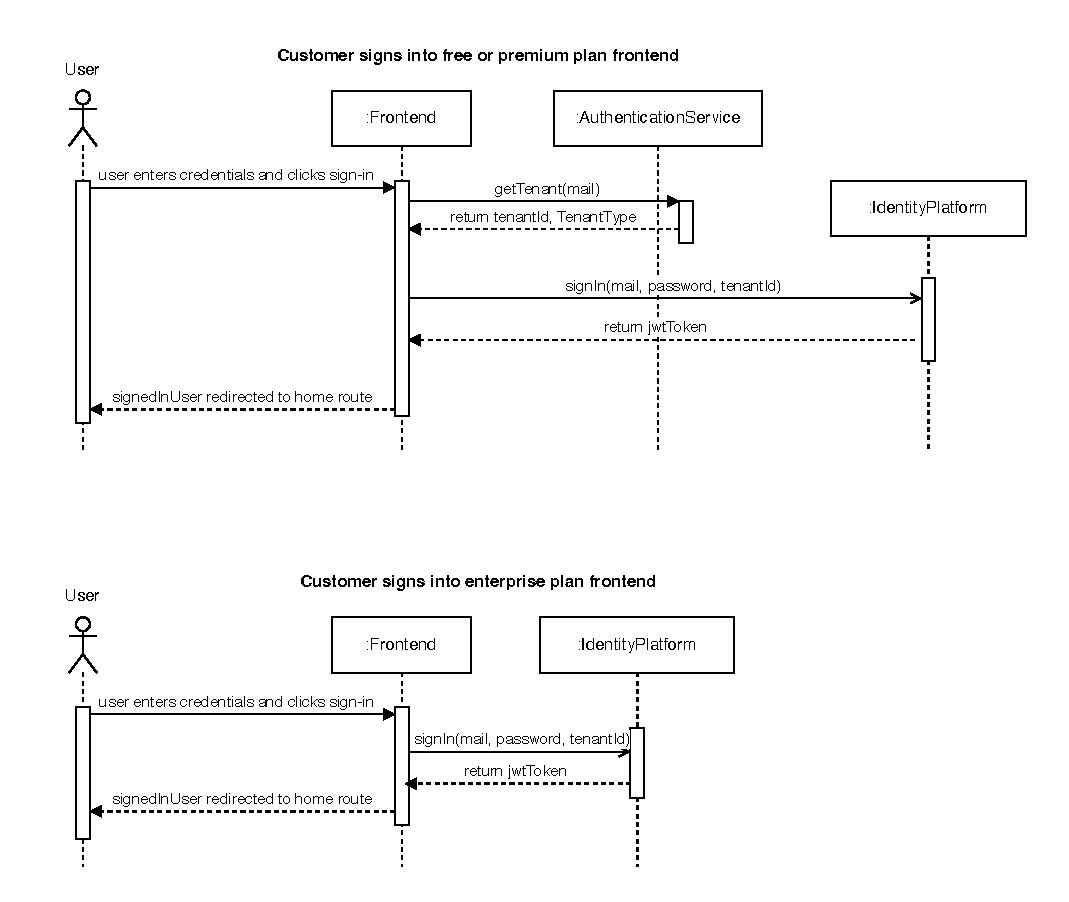
\includegraphics[width=\textwidth]{resources/03-runtime-view/pdf/authentication-sequence.pdf}
	\caption{Authentifizierungsablauf basierend auf dem Tenant-Typ}
	\label{fig:authentication-sequence}
\end{figure}

Ein besonderer Aspekt ist die Authentifizierung über den Authentication Service und die Identity Platform. Abbildung~\ref{fig:authentication-sequence} zeigt den Ablauf:
Wenn sich ein Nutzer über seine tenant-typ-spezifische Frontend-Instanz anmeldet, validiert der Authentication Service zunächst, ob der Nutzer dem entsprechenden Tenant-Typ angehört und ermittelt dessen Tenant-ID. Anschließend erfolgt die Authentifizierung über die Identity Platform. Bei erfolgreicher Authentifizierung wird der Nutzer zur zugehörigen Startseite weitergeleitet und das JWT-Token im Local Storage für die Backend-Kommunikation gespeichert.
Bei Enterprise-Tenants entfällt die Überprüfung durch den Authentication Service, da jede Enterprise-Frontend-Instanz nur von einem spezifischen Tenant genutzt wird und dessen Tenant-ID bereits in der Umgebungskonfiguration hinterlegt ist. Diese Mechanismen gewährleisten, dass sich Nutzer ausschließlich in der zu ihrem Tenant-Typ gehörenden Instanz authentifizieren können.

\begin{figure}[H]
	\centering
	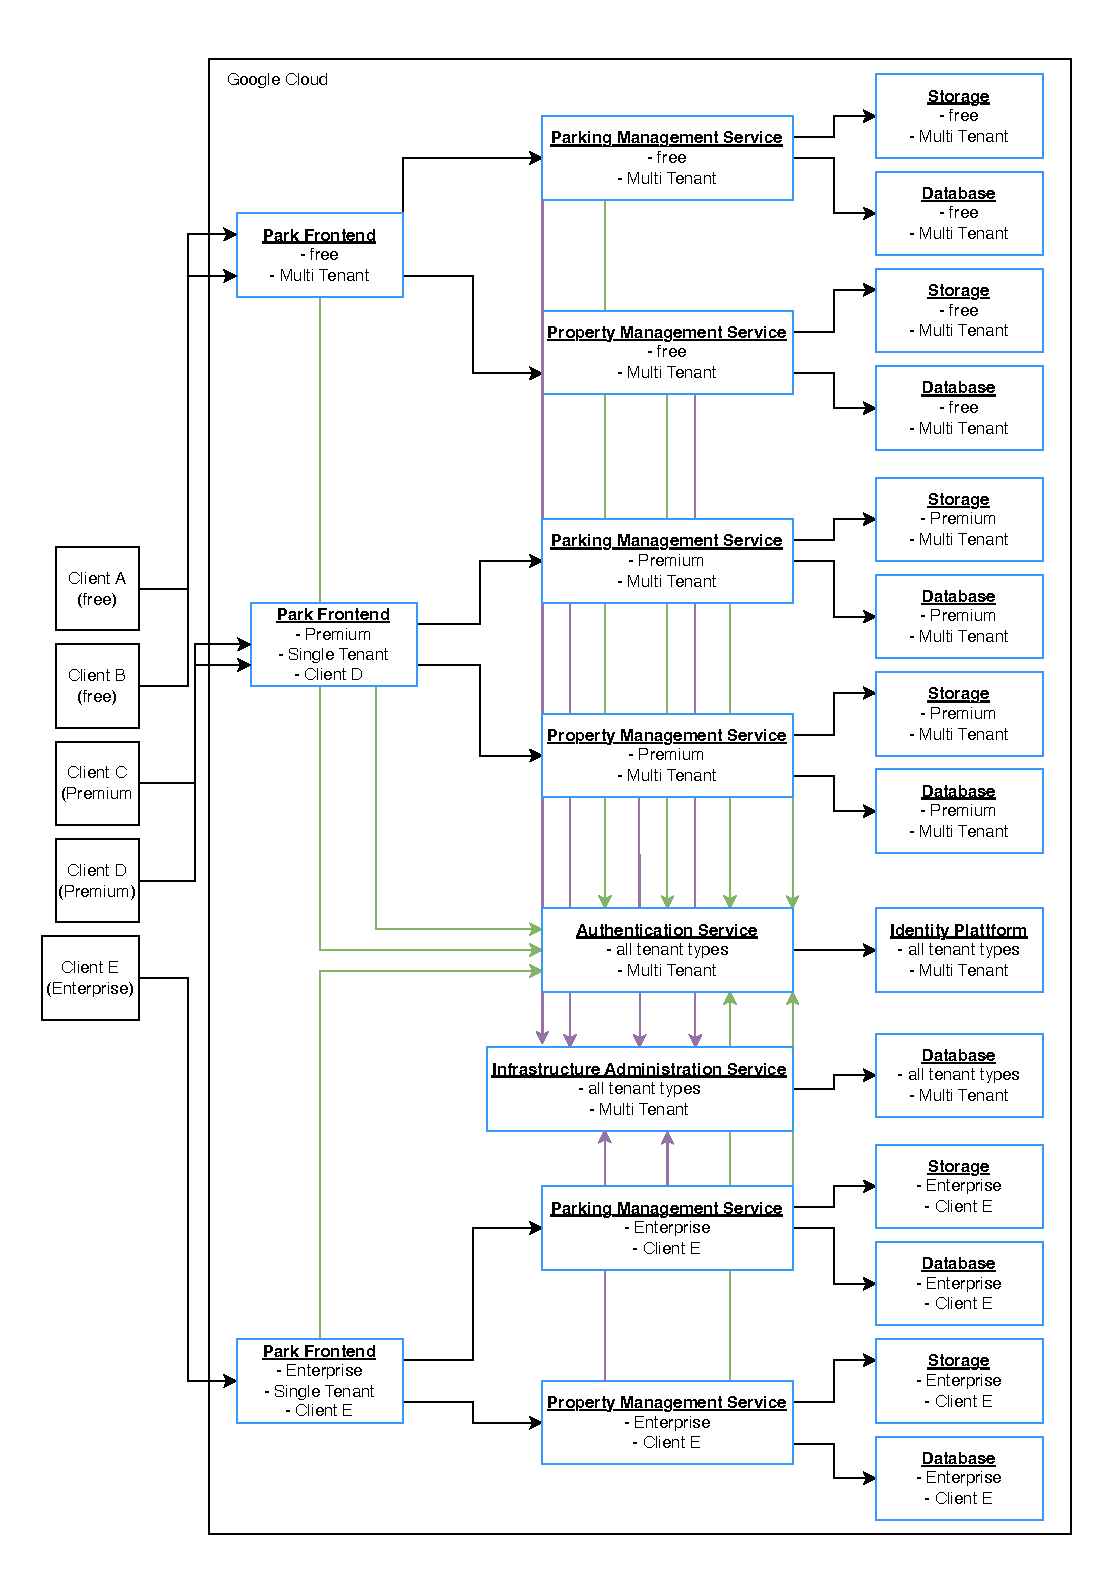
\includegraphics[width=0.95\textwidth]{resources/03-runtime-view/pdf/components-frontend-park.pdf}
	\caption{Übersicht aller Komponenten bei Interaktion mit dem PARK-Frontend unter Berücksichtigung von Multi-Tenancy}
	\label{fig:components-park-frontend}
\end{figure}

\begin{figure}[H]
	\centering
	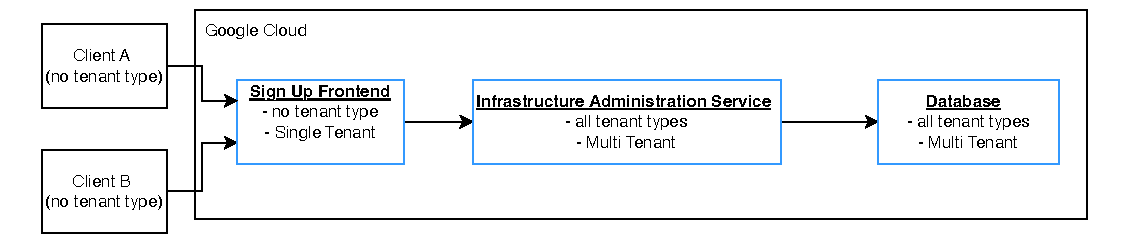
\includegraphics[width=\textwidth]{resources/03-runtime-view/pdf/components-frontend-signup.pdf}
	\caption{Übersicht aller Komponenten bei Interaktion mit dem Sign-Up-Frontend}
	\label{fig:components-signup-frontend}
\end{figure}

\subsection{Microservices}
Dieser Abschnitt beschreibt die einzelnen Microservices, die in Abbildung~\ref{fig:system-architecture} in Bezug auf ihre Komponenten und Laufzeitumgebung dargestellt sind. Die detaillierte Betrachtung der Komponenten und der Laufzeitumgebung erfolgt nicht an dieser Stelle, da diese Informationen bereits in den Abbildungen~\ref{fig:components-park-frontend}, \ref{fig:system-architecture} und~\ref{fig:components-signup-frontend} enthalten und in Kapitel~\ref{sec:development-view} beschrieben sind.

\subsubsection{Globale Microservices}
Die folgenden Microservices werden von allen Tenants gemeinsam genutzt und sind in Google Cloud Run gehostet:

\paragraph{Sign-Up Frontend}
\label{sec:signup-frontend}
\begin{itemize}
	\item Dient der Registrierung neuer Tenants und wird von allen Nutzern verwendet.
	\item Konfigurierbar über Environment-Variablen (siehe Tabelle~\ref{tab:signup-frontend-env-vars}).
	\item Automatische Skalierung durch Google Cloud Run mit den standardmäßigen Skalierungseinstellungen.
	\item Keine Individualisierungsmöglichkeiten.
	\item Sicherheitskonzept: Kein dediziertes Sicherheits-Setup erforderlich, da der Service lediglich eine Anfrage an den Infrastructure Management Service sendet, wenn sich ein neuer Tenant registriert.
	\item Kommuniziert ausschließlich mit einem Endpunkt des Infrastructure Management Services.
\end{itemize}

\paragraph{Authentication Service}
\label{sec:auth-service}
\begin{itemize}
	\item Verantwortlich für die Erstellung neuer Nutzer und Tenants sowie das Abrufen von Nutzerinformationen.
	\item Konfigurierbar über Environment-Variablen (siehe Tabelle~\ref{tab:auth-service-env-vars}).
	\item Automatische Skalierung durch Google Cloud Run.
	\item Keine Individualisierungsmöglichkeiten.
	\item Sicherheitskonzept: Der Service ist über HTTPS erreichbar und erfordert für alle Anfragen (mit Ausnahme von Anfragen zur Bestimmung des Tenant-Typs) einen Authorization Header mit einem gültigen Identity Platform JWT-Token. Durch eine IAM-Policy wird sichergestellt, dass nur der Authentication Service auf die Authentication Firestore-Datenbanken zugreifen kann.
	\item Verbindung zur Authentication Firestore-Datenbank und zur Google Cloud Identity Platform.
\end{itemize}

\paragraph{Infrastructure Management Service}
\begin{itemize}
	\item Zuständig für die Erstellung neuer Tenants, das Abrufen von Tenant-Informationen sowie die Speicherung von Analytics-Daten pro Tenant.
	\item Konfigurierbar über Environment-Variablen (siehe Tabelle~\ref{tab:infra-admin-service-env-vars}).
	\item Automatische Skalierung durch Google Cloud Run.
	\item Keine Individualisierungsmöglichkeiten.
	\item Sicherheitskonzept: Der Service ist über HTTPS erreichbar und erfordert für jede Anfrage einen Authorization Header mit einem Identity Platform JWT-Token zur Validierung. Eine IAM-Policy stellt sicher, dass ausschließlich der Infrastructure Management Service Zugriff auf die Infrastructure Management Firestore-Datenbanken und den zugehörigen Cloud Storage Bucket hat.
	\item Verbindung zur eigenen Infrastructure Firestore-Datenbank, zum Cloud Storage Bucket und zu GitHub zur Steuerung von Pipelines für die Erstellung neuer Tenants.
\end{itemize}

\subsubsection{Tenant-Typ-spezifische Microservices}
Die folgenden Microservices werden von allen Tenants eines bestimmten Tenant-Typs gemeinsam genutzt. Für jeden Tenant-Typ existiert ein separater Namespace in der Google Cloud Kubernetes Engine, in dem diese Services betrieben werden. Der Enterprise-Tenant-Typ bildet eine Ausnahme, da jeder Enterprise-Tenant über einen eigenen Namespace verfügt, weshalb die entsprechenden Services hier nicht gemeinsam genutzt werden.

\paragraph{PARK Frontend}
\begin{itemize}
	\item Benutzeroberfläche zur Verwaltung von Parkhäusern, Parkplätzen und Ladestationen, zur Anzeige von Analysen und zum Melden von Defekten.
	\item Konfigurierbar über Environment-Variablen (siehe Tabelle~\ref{tab:park-frontend-env-vars}).
	\item Skalierung durch einen Horizontal Pod Autoscaler (HPA), der auf CPU-Auslastung reagiert, sowie durch vertikale Skalierung mittels Container Resource Requests und Limits. Der HPA skaliert ab 80\% CPU-Auslastung mit einem Maximum von 10 Pods.
	\item Keine Individualisierungsmöglichkeiten. Die Darstellung des Frontends unterscheidet sich jedoch für Premium- und Enterprise-Tenants (z. B. zusätzliche Analyseseite, Sprachwahl zwischen Deutsch und Englisch).
	\item Sicherheitskonzept: Nutzer müssen sich über die Identity Platform authentifizieren. Der Service ist über HTTPS erreichbar, und durch eine Anfrage an den Authentication Service wird überprüft, ob sich nur Nutzer des entsprechenden Tenant-Typs anmelden können. Alle Anfragen an den Backend-Service erfordern einen Authorization Header mit einem Identity Platform JWT-Token. Alle Routen – mit Ausnahme von „Home“ und „Contact“ – sind nur für authentifizierte Nutzer zugänglich.
	\item Kommuniziert mit allen anderen Microservices.
\end{itemize}

\paragraph{Parking Management Service}
\begin{itemize}
	\item Schnittstelle zur Steuerung von Schranken, Bezahlterminals und Ladestationen sowie zur Bereitstellung von Belegungsstatus-Informationen für externe Monitore.
	\item Konfigurierbar über Environment-Variablen (siehe Tabelle~\ref{tab:parking-mgmt-service-env-vars}).
	\item Skalierung analog zum PARK Frontend.
	\item Keine Individualisierungsmöglichkeiten.
	\item Sicherheitskonzept: Der Service ist über HTTPS erreichbar. Für die meisten Anfragen ist ein Authorization Header mit einem Identity Platform JWT-Token erforderlich. Eine Ausnahme bildet der Endpunkt zur Abfrage des Belegungsstatus eines Parkhauses, der ohne Authentifizierung verfügbar ist. Eine IAM-Policy stellt sicher, dass nur der Parking Management Service auf die zugehörige Firestore-Datenbank zugreifen kann.
	\item Verbindung zur eigenen Parking Management Firestore-Datenbank und zum Property Management Service.
\end{itemize}

\paragraph{Property Management Service}
\begin{itemize}
	\item Zuständig für die Verwaltung von Parkhausinformationen, Defect-Reports und die Speicherung zugehöriger Bilder.
	\item Konfigurierbar über Environment-Variablen (siehe Tabelle~\ref{tab:property-mgmt-service-env-vars}).
	\item Skalierung analog zum PARK Frontend.
	\item Keine Individualisierungsmöglichkeiten.
	\item Sicherheitskonzept: Der Service ist über HTTPS erreichbar. Für alle Anfragen ist ein Authorization Header mit einem Identity Platform JWT-Token erforderlich. Eine IAM-Policy stellt sicher, dass nur der Property Management Service auf die Property Management Firestore-Datenbank und den zugehörigen Cloud Storage Bucket zugreifen kann.
	\item Verbindung zur eigenen Property Management Firestore-Datenbank, dem zugehörigen Cloud Storage Bucket und dem Parking Management Service.
\end{itemize}

\subsection{Data Stores}

\subsubsection{Globale Datastores}
Die folgenden Datenspeicher werden von den globalen Cloud-Run-Microservices genutzt:

\paragraph{Authentication Firestore}
\begin{itemize}
	\item Speicherung und Verwaltung von Nutzerdaten durch den Authentication Service.
	\item \textbf{Integritätsbedingungen:} Die Nutzer-ID, die von der Identity Platform generiert wird, ist eindeutig und wird als Primärschlüssel verwendet.
	\item \textbf{Sicherheitsrichtlinien:} Zugriff ist ausschließlich dem Authentication Service vorbehalten (IAM-Policy).
\end{itemize}

\paragraph{Infrastructure Management Firestore}
\begin{itemize}
	\item Speicherung der Anzahl der Anfragen pro Tenant zur Abrechnung sowie von Analytics-Daten pro Tenant.
	\item \textbf{Integritätsbedingungen:} Die Tenant-ID, die durch die Identity Platform generiert wird, ist eindeutig und dient als Primärschlüssel.
	\item \textbf{Sicherheitsrichtlinien:} Zugriff ist ausschließlich dem Infrastructure Management Service vorbehalten (IAM-Policy).
\end{itemize}

\paragraph{Infrastructure Management Cloud Storage Bucket}
\begin{itemize}
	\item Speicherung der Anzahl der Anfragen pro Tenant zur Abrechnung sowie von Analytics-Daten pro Tenant.
	\item \textbf{Integritätsbedingungen:} Die Tenant-ID, die durch die Identity Platform generiert wird, ist eindeutig und wird als Primärschlüssel verwendet.
	\item \textbf{Sicherheitsrichtlinien:} Zugriff ist ausschließlich dem Infrastructure Management Service vorbehalten (IAM-Policy).
\end{itemize}

\subsubsection{Tenant-Typ-spezifische Datastores}
Die folgenden Datenspeicher werden von einem tenant-typ-spezifischen Kubernetes-Namespace genutzt. Beim Enterprise-Tenant-Typ erhält jeder Tenant einen eigenen Namespace, sodass diese Datenspeicher nicht gemeinsam genutzt werden.

\paragraph{Parking Management Firestore}
\begin{itemize}
	\item Speicherung von Informationen zu Ladevorgängen, Parkhausbelegen usw.
	\item \textbf{Integritätsbedingungen:} Die Parkhaus-ID, die durch den Property Management Service generiert wird, ist eindeutig und wird als Primärschlüssel verwendet. Auch für untergeordnete Collections und Daten werden eindeutige Primärschlüssel verwendet.
	\item \textbf{Sicherheitsrichtlinien:} Zugriff ist ausschließlich dem Parking Management Service der zugehörigen Tenant-Typ-Instanz vorbehalten (IAM-Policy).
\end{itemize}

\paragraph{Property Management Firestore}
\begin{itemize}
	\item Speicherung von Informationen zu Parkhäusern und Defect Reports.
	\item \textbf{Integritätsbedingungen:} Die Parkhaus-ID und Defect-ID, die durch den Property Management Service generiert werden, sind eindeutig und werden als Primärschlüssel verwendet.
	\item \textbf{Sicherheitsrichtlinien:} Zugriff ist ausschließlich dem Property Management Service der zugehörigen Tenant-Typ-Instanz vorbehalten (IAM-Policy).
\end{itemize}

\paragraph{Cloud Storage Defects Bucket}
\begin{itemize}
	\item Speicherung von Bildern zu Defect Reports.
	\item \textbf{Integritätsbedingungen:} Bilder werden über eine signierte URL hochgeladen, die von der Cloud bereitgestellt wird. Dies gewährleistet, dass die Bilder mit einem eindeutigen Primärschlüssel abgelegt werden.
	\item \textbf{Sicherheitsrichtlinien:} Zugriff ist ausschließlich dem Property Management Service der zugehörigen Tenant-Typ-Instanz vorbehalten (IAM-Policy). Nur dieser Service kann Anfragen zur Erstellung einer neuen signierten URL stellen.
\end{itemize}

\subsection{Cloud Functions}
Jeder Tenant besitzt eine Cloud Function, die ausgelöst wird, wenn ein neuer Defect Report in der Property Management Firestore-Datenbank erstellt wird. Diese Cloud Function benachrichtigt den Property Management Service, sodass dieser den neuen Defect Report verarbeiten kann.
